\chapter{Logische Grundbegriffe}\label{logik}

In diesem Kapitel sollen die für spätere Ausführungen benötigten Grundbegriffe der formalen Logik (insbesondere der Prädikatenlogik) eingeführt werden. Dabei soll auf Syntax und Semantik der Prädikatenlogik, Hornklauseln, Unifikation und Resolutionsverfahren sowie -strategien eingegangen werden.

\section{Prädikatenlogik}\label{praedlog}
Die Prädikatenlogik ist eine Erweiterung der Aussagenlogik, bei der Literale nicht als Aussagen mit einem fixen Wahrheitswert interpretiert werden, sondern als Prädikate, deren Wahrheitswert von ihren Argumenten abhängt. In diesem Abschnitt werden Syntax und Semantik der Prädikatenlogik eingeführt. Die hier verwendete Darstellung von Formeln ist umfangreicher in \cite{beckstein} zu finden.

\subsection{Syntax}
Formeln der Prädikatenlogik sind Wörter über dem Alphabet

\begin{equation}
  \Sigma = V \cup F \cup P \cup J \cup Q \cup I
\end{equation}
wobei

\begin{itemize}
\item $V = \left \{ x_{1},...,x_{n} \right \}$ (Variablensymbole),
\item $F$ eine Menge von n-stelligen Funktionssymbolen (einschließlich von 0-stelligen Funktionen, den sog. Konstanten),
\item $P$ eine Menge von n-stelligen Prädikatssymbolen,
\item $J = \left \{ \neg , \wedge , \vee , \Rightarrow ,\Leftrightarrow   \right \}$ (Junktoren),
\item $Q = \left \{ \exists , \forall \right \}$ (Quantoren),
\item $I = \left \{ :, , , (, )\rigth \}$ (Interpunktionen)
\end{itemize}
\noindent
sind.

Prädikatesymbole und Funktionssymbole bilden die Signatur einer prädikatenlogischen Sprache. Sie sind von der Anwendung abhängig und müssen disjunkt sein. Alle Funktions- oder Prädikatsymbole müssen von den in den anderen Teilmengen vorkommenden Symbolen verschieden sein.

Aus Variablen, Konstanten und Funktionssymbolen lassen sich Terme bilden.

\begin{leftbar}
  \begin{definition}[Terme]\label{terme}
    \begin{description}
    \item[(IA)] Variablen und Konstantensymbole sind Terme \newline
    \item[(IS)] Sind $t_{1},...,t_{n}$ Terme und $f$ ein Funktionssymbol, ist auch $f(t_{1},...,t_{n})$ ein Term.
    \end{description}
  \end{definition}
\end{leftbar}
\noindent
Aus Termen und einem Prädikatsymbol lassen sich atomare Formeln bilden.

\begin{leftbar}
  \begin{definition}[atomare Formel]
    \newline
    Seien  $t_{1},...,t_{n}$ Terme und $P$ ein Prädikatssymbol. Dann ist $P(t_{1},...,t_{n})$ eine atomare Formel. Wir nennen atomare Formeln auch kurz Atome    
  \end{definition}
\end{leftbar}
\noindent
Durch das Verknüpfen von atomaren Formeln mittels Junktoren und das Quantifizieren von Variablen lassen sich zusammengesetzte Formeln bilden.

\begin{leftbar}
  \begin{definition}[Formeln]
    \begin{description}
    \item[(IA)] Atomare Formeln sind Formeln \newline
    \item[(IS)] Sind $F$ und $G$ Formeln und $x_{1},...,x_{n}$ Variablen, dann sind auch
      \begin{itemize}
      \item $\neg F$ (Negation),
      \item $F \wedge G$ (Konjunktion),
      \item $F \vee G$ (Disjunktion),
      \item $F \Rightarrow G$ (Implikation),
      \item $F \Leftrightarrow G$ (Äquivalenz),
      \item $\forall x_{1},...,x_{n}:F$ und
      \item $\exists x_{1},...,x_{n}:F$
      \end{itemize}
      Formeln.
    \end{description}
  \end{definition}
\end{leftbar}
\noindent
Mit diesen drei Definitionen lassen sich alle Formeln der Prädikatenlogik bilden. Der Begriff des Literals erlaubt uns für die folgenden Ausführungen eine kompaktere Darstellung von Formeln.

\begin{leftbar}
  \begin{definition}[Literal]
    \newline
    Ein Literal ist eine atomare Formel (positives Literal) oder eine negierte atomare Formel (negatives Literal).
  \end{definition}
\end{leftbar}

Das in dieser Arbeit entwickelte Schlussfolgerungssystem arbeitet auf einer bestimmten Teilmenge prädikatenlogischer Formeln, die als Hornklauseln bezeichnet werden. Wir betrachten zunächst die allgemeine Darstellung prädikatenlogischer Formeln als Menge von Klauseln.

\begin{leftbar}
  \begin{definition}[Konjunktive und Klauselnormalform]
    \newline
    Eine Formel ist in konjunktiver Normalform, wenn sie nur aus einer Konjunktion von Disjunktionen von Literalen besteht.
    \newline
    Sind $L_{11},...,L_{mn}$ Literale (für $m,n \geq 1$) ist die Formel
    \begin{equation}
      ((L_{11} \vee ... \vee L_{1n}) \wedge ... \wedge (L_{m1} \vee ... \vee L_{mn}))
    \end{equation}
    in konjunktiver Normalform.
    \newline
    Die Klauselnormalform ist eine Mengendarstellung einer Formel in konjunktiver Normalform.
    \begin{equation}
      \left \{ \left \{L_{11},...,L_{1n}\right \},...,\left \{ L_{m1},...,L_{mn}\right \} \right \}
    \end{equation}
    \newline
    Ein Element der Klauselnormalform nennen wir Klausel.
  \end{definition}
\end{leftbar}
\noindent
Jede prädikatenlogische Formel lässt sich in eine erfüllbarkeitsäquivalente Formel in Klauselnormalform überführen.

\begin{leftbar}
  \begin{definition}[Hornklausel]
    \newline
    Eine Hornklausel ist eine Klausel die höchstens ein positives Literal enthält.
  \end{definition}
\end{leftbar}
\noindent
Hornklauseln lassen sich auf zwei verschiedene Arten bequem als prädikatenlogische Formeln darstellen.

\begin{leftbar}
  \begin{definition}[Fakten- und Regelform]
    \newline
    Eine Formel ist in Faktenform, wenn sie lediglich aus einem positiven Literal besteht.
    \begin{equation}
      P(x)
    \end{equation}
    \newline
    Eine Formel ist in Regelform, wenn sie aus einer Implikation zwischen einer Konjunktion und einem positven Literal besteht
    \begin{equation}
      Q_1(x) \wedge ... \wedge Q_n(x) \Rightarrow P(x)
    \end{equation}
  \end{definition}
\end{leftbar}
\noindent
Um Sinnvoll über die Bedeutung einer Formel sprechen zu können, müssen zwei Klassen von Variablen innerhalb einer Formel unterschieden werden.
\newpage
\begin{leftbar}
  \begin{definition}[freie und gebundene Variablen]
    \newline
    Wird eine Variable $x$ in einer Formel $F$ durch einen Quantor ($\forall$,$\exists$) gebunden, heißt $x$ in $f$ \textbf{gebundene Variable}.\newline
    \newline
    Alle Variablen die in einer Formel nicht gebunden sind, heißen \textbf{freie Variablen}.
    \newline
    Eine Formel die keine freien Variablen enthält, nennen wir geschlossene Formel.
  \end{definition}
\end{leftbar}
\noindent
Wir betrachten von nun an nur noch geschlossene Formeln und gehen davon aus, dass alle Variablen durch einen Allquantor gebunden sind. Man spricht dann vom universellen Abschluss einer Formel.

\subsection{Semantik}
Um einer prädikatenlogischen Sprache eine Semantik zuzuordnen, muss der Definitionsbereich (das sog. Universum) bekannt sein und den Symbolen der Signatur müssen Elemente über diesem Universum zugeordnet werden.

\begin{leftbar}
  \begin{definition}[Interpretation]
    \newline
    Eine Interpretation $\mathcal{I} = \left ( \mathcal{U},\mathcal{F},\mathcal{P},\mathcal{V} \right )$ besteht aus
    \begin{itemize}
    \item dem Universum $\mathcal{U}$,
    \item einer Funktion $\mathcal{F}$, die jedem Funktionssymbol eine Funktion über $\mathcal{U}$ zuordnet,
    \item einer Funktion $\mathcal{P}$, die jedem Prädikatsymbol eine Relation über $\mathcal{U}$ zuordnet und
      \item einer Funktion $\mathcal{V}$, die jeder Variable ein Element aus $\mathcal{U}$ zuordnet.
    \end{itemize}
  \end{definition}
\end{leftbar}
\noindent
Die Funktion $\mathcal{V}$ lässt sich auf Funktionsterme ausweiten. Die Bewertung von Termen ergibt sich dann aus der Instantierung von Funktions- und Variablensymbolen.

\begin{equation}
  \mathcal{V}(f(t_1,...,t_n)) = \mathcal{F}(f)(\mathcal{V}(t_1),...,\mathcal{V}(t_n))
\end{equation}
\noindent
Daraus ergibt sich direkt der Wahrheitswert atomarer Formeln.

\begin{equation}
  R(t_1,...,t_n) \text{ ist wahr gdw. } (\mathcal{V}(t_1),...,\mathcal{V}(t_n)) \in \mathcal{P}(R)
\end{equation}
\noindent
Der Wahrheitswert mittels Junktoren zusammengesetzter Formeln ergibt sich auch der üblichen Interpretation der Junktoren.
\newline
\begin{center}
\begin{tabular}{ l l | c | c | c | c | c }
  $F$ & $G$ & $\neg F$ & $F \wedge G$ & $F \vee G$ & $F \Rightarrow G$ & $F \Leftrightarrow G$ \\
  \hline
  falsch & falsch & wahr & falsch & falsch & wahr & wahr \\
  falsch & wahr & wahr & falsch & wahr & wahr & falsch \\
  wahr & falsch & falsch & falsch & wahr & falsch & falsch\\
  wahr & wahr & falsch & wahr & wahr & wahr & wahr\\
\end{tabular}
\end{center}
\newline
\newline
\noindent
Der Wahrheitswert quantifizierter Formeln ergibt sich aus der Bedeutung der Quantoren.

\begin{leftbar}
  \begin{definition}[All- und Existenzquantoren]
    \newline
    Eine Formel der Form $\forall x:F$ ist wahr gdw. alle Variablenbelegungen, die sich höchstens in der Belegung von $x$ unterscheiden, $F$ wahr machen.
    \newline
    \newline
    Eine Formel der Form $\exists x:F$ ist wahr gdw. $\neg \forall x: \neg F$ wahr ist.
  \end{definition}
\end{leftbar}
\noindent
Ist eine Formel $F$ unter der Interpretation $\mathcal{I}$ wahr, schreiben wir
\begin{equation}
  \mathcal{I} \models F
\end{equation}
\noindent
Wir nennen $\mathcal{I}$ auch Modell der Formel $F$.

Über den Wahrheitswert einer Formel unter einer Interpretation lassen sich Erfüllbarkeit und Folgerung definieren.

\begin{leftbar}
  \begin{definition}[Erfüllbarkeit]
    \newline
    Eine Formel F heißt erfüllbar gdw. eine Interpretation $\mathcal{I}$ existiert, sodass
    \begin{equation}
      \mathcal{I} \models F
    \end{equation}
    \noindent
    Existiert keine solche Interpretation, heißt F unerfüllbar.
  \end{definition}
\end{leftbar}

\begin{leftbar}
  \begin{definition}[Folgerung]
    \newline
    Sei $\Gamma$ eine Menge geschlossener Formeln und $F$ eine geschlossene Formel. Wir bezeichnen $F$ als Folgerung von $\Gamma$ falls für jede Interpretation $\mathcal{I}$ gilt
    \begin{equation}
      \text{falls } \mathcal{I} \models \Gamma, \text{dann } \mathcal{I} \models F
    \end{equation}
    Wir schreiben dann,
    \begin{equation}
       \Gamma \models F
    \end{equation}
  \end{definition}
\end{leftbar}
\noindent
Eine für diese Arbeit wichtige Konsequenz ist, das für eine Menge geschlossener Formeln $\Gamma$ und eine geschlossene Formel $F$ gilt, dass

\begin{equation}
  \Gamma \cup \left \{ \neg F \right \} \text{ ist unerfüllbar gdw. } \Gamma \models F
\end{equation}
\noindent
Aufgabe eines Schlussfolgerungssystems ist es nun für eine gegebene Menge an Formel (die Axiome) und eine weitere Formel (die Behauptung) zu entscheiden, ob die Behauptung aus den Axiomen folgt. Idealerweise liefert das System dabei auch die in der Interpretation verwendete Variablenbelegung.

Da dies direkt praktisch nicht automatisierbar ist, wird ein operationelles Verfahren, ein sogenannter Kalkül benötigt. Ein Kalkül besteht aus einer Menge von Axiomen und Schlussregeln durch die es schrittweise möglich ist, die Folgerungsbeziehung zwischen einer Menge von Formeln und einer Behauptung zu beweisen.

\subsection{Resolutionskalkül}\label{res}
Der Resolutionskalkül liefert ein formales Verfahren, um eine solche Folgerungsbeziehung zu beweisen. Die Resolutionsregel basiert auf dem Instanzieren von Variablen mit konkreteren Termen wie Konstanten oder Funktionen. Das Instanzieren kann als Anwendung einer Substitution betrachtet werden. 

\begin{leftbar}
  \begin{definition}[Substitution auf Termen]
    \newline
    Sei $T$ die Menge aller Terme und $V$ die Menge aller Variablen. Eine Substitution ist eine Abbildung $\sigma : T \rightarrow T$ sodass,

    \begin{enumerate}
    \item $\sigma(c) = c$ für alle Konstanten
    \item $\sigma(f(t_1,...,t_n)) = f(\sigma(t_1),...,\sigma(t_n))$
    \item $\left \{ x \in V | \sigma(x) \neq x \right \}$ ist endlich
    \end{enumerate}
    \newline
    Eine Substitution heißt Idempotent wenn $\sigma(t) = \sigma(\sigma(t))$
  \end{definition}
\end{leftbar}
\noindent
Idempotente Substitutionen können auch als Menge von Paaren dargestellt werden

\begin{equation}
  \left \{ x_1 \leftarrow t_1, ... , x_n \leftarrow t_n \right \}
\end{equation}
\noindent
Wenn Mehrdeutigkeiten ausgeschlossen sind, schreiben wir statt $\sigma(T)$ auch einfacher $\sigma T$

Die Substitutionsabbildung lässt sich wie folgt auf Formeln erweitern.
\begin{eqnarray}
  \sigma P(t_1,...,t_n) = P(\sigma t_1,...,\sigma t_n) \\
  \sigma \neg P(t_1,...,t_n) = \neg P(\sigma t_1,...,\sigma t_n) \\
  \sigma \left \{ L_1,...,L_n \right \} = \left \{ \sigma L_1,..., \sigma L_n \right \}
\end{eqnarray}

Unifikation beschreibt die systematische Vereinheitlichung von zwei Atomen durch Anwenden von Substitutionen. Zwei Atome $P(s_1,...,s_n)$ und $Q(t_1,...,t_n)$ sind dabei unifizierbar, wenn $P = Q$ und die beiden Termlisten $(s_1,...,s_n)$ und $(t_1,...,t_n)$ unifizierbar sind.

\begin{leftbar}
  \begin{definition}[Unifikator]
    \newline
    Eine Substitution $\sigma$ heiß Unifikator zweier Terme $s$ und $t$, wenn $\sigma s = \sigma t$.
    \newline
    Ein Unifikator $\sigma$ heißt allgemeinster Unifikator (mgu = most general unifier), falls es für jeden weiteren Unifikator $\tau$ eine Substitution $\lambda$ gibt, sodass $\tau = \lambda \sigma$
  \end{definition}
\end{leftbar}

Die Resolutionsregel beschreibt, wie aus zwei Klauseln einer Klauselmenge eine neue Klausel abgeleitet werden kann. Sie basiert auf dem Modus Ponens.

\begin{equation}
  \frac{F \;\; \; \;  F \Rightarrow G }{G}
\end{equation}
\noindent
Gilt sowohl die Formel $F$ als auch, das $F$ $G$ impliziert, so gilt auch $G$.

Die Resolutionsregel ist eine Verallgemeinerung des Modus Ponens. Sei $\sigma$ ein mgu für $F$ und $F'$. Dann gilt

\begin{equation}
  \frac{K_1 = \left \{ F ,L_1,...L_n \right \} \;\; \; \;  K_2 = \left \{ \neg F' ,G_1,...,G_m \right \} }{R = \sigma \left \{ L_1,...,L_n,G_1,...,G_n \right \}}
\end{equation}
\noindent
Wir nennen die Klauseln $K_1$ und $K_2$ Elternklauseln der Resolvente $R$.

\begin{leftbar}
\begin{satz}
  Die Resolutionsregel ist korrekt.
\end{satz}
\end{leftbar}
\noindent
\textbf{Beweis:}

Sei $\mathcal{I}$ eine Interpretation unter der $(F \vee L_1 \vee ... \vee L_n) \wedge (\neg F' \vee G_1 \vee ... \vee G_m)$ wahr ist und $\sigma$ ein Unifikator für $F$ und $F'$. Dann sind

\begin{itemize}
\item $(\sigma F \vee \sigma L_1 \vee ... \vee \sigma L_n)$ und
\item $(\neg \sigma F' \vee \sigma G_1 \vee ... \vee \sigma G_m)$
\end{itemize}
unter $\mathcal{I}$ wahr. $\sigma F$ ist unter $\mathcal{I}$ entweder wahr oder falsch.

Falls $\sigma F$ unter $\mathcal{I}$ wahr ist, ist $\neg \sigma F'$ unter $\mathcal{I}$ falsch (da $\sigma F = \sigma F'$). Dann ist $(G_1 \vee ... \vee G_m)$ unter $\mathcal{I}$ wahr. Also ist auch $(G_1 \vee ... \vee G_m \vee L_1 \vee ... \vee L_n)$ unter $\mathcal{I}$ wahr.

Falls $\sigma F$ unter $\mathcal{I}$ falsch ist, ist $(L_1 \vee ... \vee L_n)$ unter $\mathcal{I}$ wahr. Also ist auch $(G_1 \vee ... \vee G_m \vee L_1 \vee ... \vee L_n)$ unter $\mathcal{I}$ wahr.
\hfill $\Box$\\
\newline
\noindent
Durch Anwendung der Resolutionsregel auf zwei Klauseln der Form

\begin{equation}
  \left \{ F \right \} \; \; \; \left \{ \neg F' \right \}
\end{equation}
\noindent
mittels eines Unifikators für $F$ und $F'$ ist die Resolvente leer. Die leere Klausel lässt sich nur aus zwei widersprüchlichen Klauseln, die unter keiner Interpretation den gleichen Wahrheitswert haben können, bilden.

\begin{leftbar}
  \begin{definition}[Ableitbarkeit]
    \newline
    Kann durch wiederholte Anwendung der Resolutionsregel auf Klauseln $K_1,...,K_n$ eine Klausel $K$ gebildet werden, ist $K$ aus $K_1,...,K_n$ ableitbar. Wir schreiben dann
    \begin{equation}
      K_1,...,K_n \vdash K
    \end{equation}
  \end{definition}
\end{leftbar}
\noindent
Lässt sich durch wiederholte Anwendung der Resolutionsregel auf Klauseln einer Klauselmenge die leere Klausel ableiten, entspricht dies einem Widerspruch und beweist die Unerfüllbarkeit der initialen Klauselmenge.

Ist nun eine Menge von geschlossenen Formeln $\Gamma$ und eine geschlossene Formel $F$ gegeben, beweist eine Resolutionsbeweis, der die Unerfüllbarkeit der Klauselmenge $\Gamma \cup \left \{ \neg F \right \}$ beweist, die Folgerung von $F$ aus $\Gamma$

Zusammen mit der Faktorisierungsregel, die hier nicht näher betrachtet wird, bildet die Resolutionsregel den Resolutionskalkül.

\begin{leftbar}
  \begin{satz}[Widerlegungsvollständigkeit]
    \newline
    Der Resolutionskalkül ist widerlegungsvollständig, d. h. für eine Menge geschlossener Formeln $\Gamma$ und eine Behauptung $F$ gilt
    \begin{equation}
      \Gamma \models F \; gdw.\; \Gamma \cup \left \{ \neg F \right \} \vdash \left \{ \right \}
    \end{equation}
\end{satz}
\end{leftbar}
\noindent

\section{Resolutionsstrategien}
Aufgrund der Widerlegungsvollständigkeit eignet sich der Resolutionskalkül als Widerlegungsverfahren für die Prädikatenlogik. Die Resolutionsregel gibt allerdings nur an, wie aus zwei Klauseln eine neue Klausel abgeleitet werden kann. Die Frage, welche zwei Klauseln für einen Resolutionschritt herangezogen werden sollen, ist entscheidend für eine effektive und effiziente Ableitung der leeren Klausel. Resolutionstrategien liefern eine Antwort auf diese Frage.

Für Mengen von Hornklauseln existiert mit der SLD-Resolution eine korrekte und widerlegungsvollständige Resolutionsstrategie.
Im Folgenden werden die grundlegenden Strategien für die SLD-Resolution vorgestellt.

\subsection{lineare Resolution}
Bei linearen Resolutionsstrategien ist eine der beiden Elternklauseln immer die Resolvente aus dem vorherigen Resolutionschritt. Die zweite Elternklausel ist frei zu wählen.

Ist zum Beispiel folgende Klauselmenge gegeben
\begin{equation}
  \left \{ \left \{ P(x,y), Q(x) \right \}^{1}, \left \{ \neg P(f(a),y), R(b) \right \}^{2}, \left \{ \neg Q(f(a)) \right \}^{3}, \left \{ \neg R(x) \right \}^{4} \right\}
\end{equation}
\noindent
wobei $x$ und $y$ Variablen und $a$ und $b$ Konstanten sind, ist
\begin{flalign*}
  & \left \{ Q(f(a)), R(b) \right \}^{5} & \text{ Resolvente aus Klausel } 1 \text{ und } 2; mgu = \left \{ x \leftarrow f(a) \right \} \\
  & \left \{ R(b) \right \}^{6} & \text{ Resolvente aus Klausel } 5 \text{ und } 3; mgu = \left \{ \right \} \\
  & \left \{  \right \} & \text{ Resolvente aus Klausel } 6 \text{ und } 4; mgu = \left \{ x \leftarrow b \right \}
\end{flalign*}
\noindent
ein linearer Resolutionsbeweis.

\subsection{Set of Support Strategie}
Zur Einschränkung des Suchraums wird bei Verwendung der Set of Support Strategie eine Teilmenge $T$ der initialen Klauselmenge $K$ gewählt, sodass $K \setminus T$ erfüllbar ist. Im Resolutionsbeweis relativ zur Stützmenge $T$, dürfen dann nie zwei Klauseln aus $K \setminus T$ miteinander resolviert werden.

Legt man fest, dass die Menge $T$ nur die negierte Behauptung enthält, werden nie zwei Axiome der initialen Klauselmenge miteinander resolviert.

\subsection{SLD-Resolution}
Die SLD-Resolution (SLD = linear resolution with selection function for definite clauses) ist eine lineare Set of Support Resolution. Dabei wird zusätzlich die Einschränkung getroffen, dass in jedem Schritt eine Klausel der initialen Klauselmenge an der Resolution beteiligt ist. Diese Einschränkung wird als Input Restriktion bezeichnet. In einem SLD Resolutionsbeweis wird also, beginnend mit der initialen Zielklausel, eine Zielklausel mit einem Axiom der initialen Klauselmenge resolviert.

Der Suchraum einer SLD-Resolution entspricht einem Baum, dessen Knoten Zielklauseln sind. Die Nachfolger eines Knotens sind Zielklauseln, die durch einen Resolutionsschritt mit einem Axiom der initialen Klauselmenge entstehen.

Sei folgende Hornklauselmenge gegeben.

\begin{flalign*}
\left \{ & \left \{ vater(paul,klaus) \right \}^{1}, \left \{ vater(klaus,steven) \right \}^{2}, \left \{ vater(paul,peter) \right \}^{3},&\\
         & \left \{ großvater(x,y), \neg vater(x,z), \neg vater(z,y) \right \}^{4}, \left \{ \neg großvater(x,steven) \right \}^{5} \left. \right \}
\end{flalign*}
\noindent
Ist Klausel fünf die initiale Zielklausel, ergibt sich der SLD-Baum in Abbildung \ref{sld-baum}.

\begin{figure} %[hbtp]
	\centering
		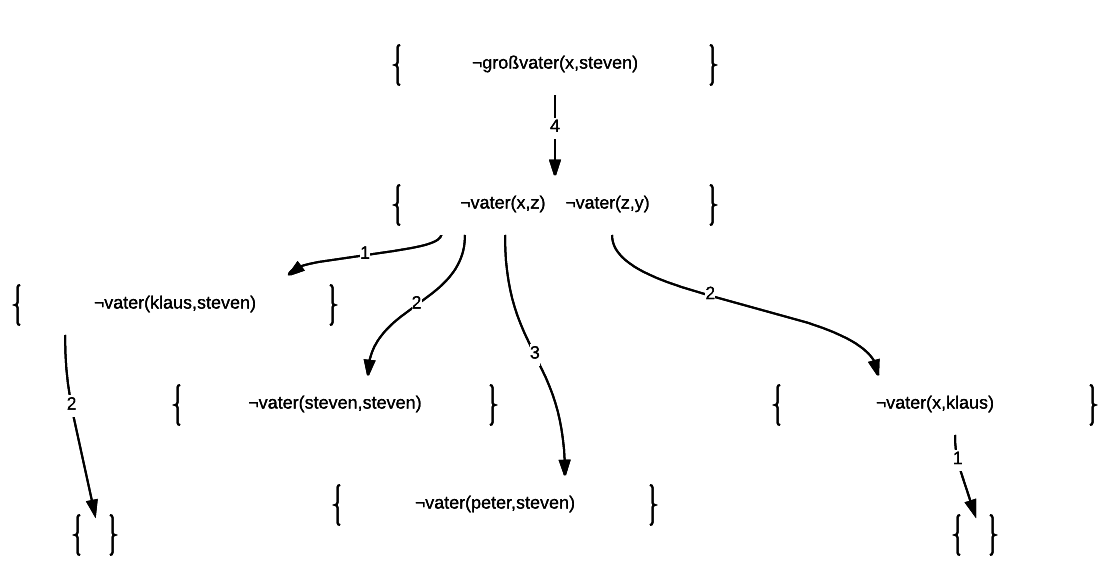
\includegraphics[scale=.9]{/home/steven/dev/lisp/cl-reason/doc/images/sld-tree.png}
	\caption{SLD-Baum}
	\label{sld-baum}
\end{figure}

Ein Resolutionsbeweis nach SLD-Strategie ist ein Wurzelpfad im SLD-Baum. Die SLD-Resolution ist widerlegungsvollständig für Mengen von Hornklauseln.
